%!TEX root = JakubJedryszek-MasterThesis.tex

\cleardoublepage


\chapter{PCA pump prototype implementation and code generation}
\label{pcapumpimpl}

This chapter describes running SPARK Ada programs on BeagleBoard-xM platform (\ref{pcapump:beagleboard}), implementation details of PCA pump prototype (\ref{pcapumpimpl:manual})) and code generation from simplified AADL/BLESS models of PCA pump (\ref{pcapumpimpl:codegen}). All programs presented in this section works the same on Intel processor (PC or MacBook) and on BeagleBoard-xM (ARM device).


\section{Running SPARK Ada programs on BeagleBoard-xM}
\label{pcapumpimpl:beagleboard}

To run SPARK Ada program on BeagleBoard-xM, it has to be cross-compiled. As an IDE for SPARK Ada development, GNAT Programming Studio (GPS) is used (see section \ref{background:spark:gps}). To create "Hello, World!" application, new Ada project has been created (choosing Project/New... from the menu). Then main.adb file, with procedure Main printing "Hello, World!" in standard output, was added. The code is presented in listing \ref{listing:HelloWorld}. It is valid Ada 2005 and Ada 2012 code.

\begin{lstlisting}[language=ada, frame=single, gobble=0, caption={"Hello World" in Ada}, label={listing:HelloWorld}]
with Ada.Text_IO;

procedure Main
is
begin
    Ada.Text_IO.Put_Line("Hello, World!");    
end Main;
\end{lstlisting} 


The main file has to be always specified in project file (\lstinline{.gpr}) in order to compile and link application, which can be runnable. It can be done in Project/Edit Project Properties (figure \ref{figure:editprojectproperties}), tab: Main files (figure \ref{figure:mainfiles}) or directly in project file (\lstinline{.gpr}).

\begin{figure}[ht]%t=top, b=bottom, h=here
    \begin{center}
    	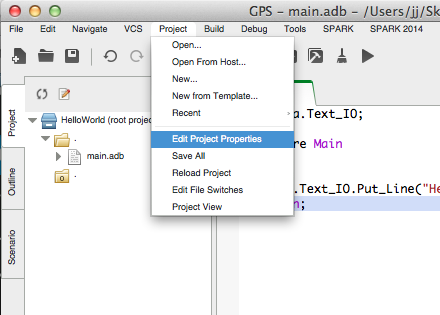
\includegraphics[width=3.2in]{figures/EditProjectProperties.png}    	
    \end{center}
    \caption{Edit Project Properties}
    \label{figure:editprojectproperties}
\end{figure}

\begin{figure}[ht]%t=top, b=bottom, h=here
    \begin{center}
    	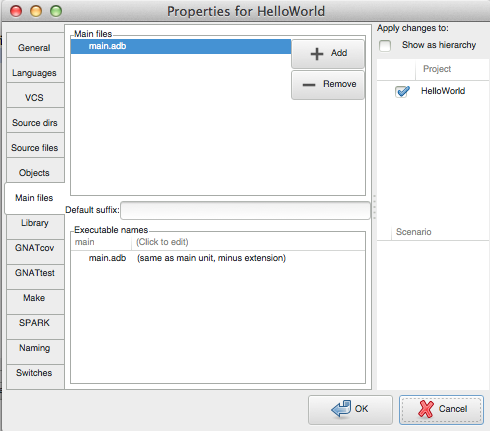
\includegraphics[width=3.2in]{figures/Properties-MainFiles.png}    	
    \end{center}
    \caption{Project Main files}
    \label{figure:mainfiles}
\end{figure}

To enable cross-compilation, for current version of cross-compiler, environmental variable \lstinline{\$ENV_PREFIX} has to be set to directory, which contains \lstinline{/lib} and \lstinline{/usr} directories. Latter should also contains \lstinline{/usr/lib} and \lstinline{/usr/include} subdirectories. After mentioned directories has been copied into \lstinline{/home/super/angstrom-arm} directory, \lstinline{\$ENV_PREFIX} has been exported with following command: \lstinline{export ENV_PREFIX=/home/super/angstrom-arm}. Entire project can be compiled and linked with following command: \lstinline{arm-linux-gnueabi-gnatmake -d -Phelloworld.gpr} (where \lstinline{helloworld.gpr} is GNAT Programming Studio project file). Additional flags can be specified in command line or directly in project file (manually or through GNAT Programming Studio Interface).

More complex example, which takes advantage of SPARK contracts is presented in section \ref{pcapumpimpl:beagleboard:odometer}.

\subsection{Odometer}
\label{pcapumpimpl:beagleboard:odometer}

Odometer is a simple SPARK Ada program, which implements basic functions of standard Odometer. Listing \ref{listing:Odometer2005} shows Odometer in SPARK 2005. In addition to \lstinline{Odometer}

\singlespacing
\begin{lstlisting}[language=ada, frame=single, gobble=0, caption={SPARK 2005 code: Odometer}, label={listing:Odometer2005}]
	package Odometer
	--# own
	--# Trip,        -- number of meters so far on this trip (can be reset to 0).
	--# Total        -- total meters traveled of vehicle since the last factory-reset.
	--#   : Natural; -- has range 0 .. Integer'Last.
	--# initializes Trip,
	--#             Total;
	is
	    procedure Zero_Trip; -- sets Trip to 0 and clears all saved Trip marks.
	    --# global out Trip;
	    --# derives Trip from ;
	    --# post Trip = 0;
	    
	    function Read_Trip return Natural; -- returns value of Trip.
	    --# global in Trip;
	    --# return Trip;
	    
	    function Read_Total return Natural; -- returns value of Total
	    --# global in Total;
	    --# return Total;
	    
	    procedure Inc; -- increments each of Trip and Total by 1.
	    --# global in out Trip, Total;
	    --# derives Trip from Trip & Total from Total;
	    --# pre Trip < Integer'Last and Total < Integer'Last;
	    --# post Trip = Trip~ + 1 and Total = Total~ + 1;	    
	end Odometer;

	package body Odometer is
	    Trip : Natural := 0;
	    Total : Natural := 0;
	    
	    procedure Zero_Trip is
	    begin
	        Trip := 0;
	    end Zero_Trip;
	    
	    function Read_Trip return Natural is
	    begin
	        return Trip;
	    end Read_Trip;
	    
	    function Read_Total return Natural is
	    begin
	        return Total;
	    end Read_Total;
	    
	    procedure Inc is
	    begin
	        Trip := Trip + 1;
	        Total := Total + 1;
	    end Inc;
	end Odometer;
\end{lstlisting} 
\doublespacing

There are 4 subprograms (2 procedures and 2 functions), which are globally available (through other packages and program units):
\begin{itemize}
    \item \lstinline{Zero_Trip} procedure - reset Odometer to 0
    \item \lstinline{Read_Trip} function - returns current distance
    \item \lstinline{Read_Total} function - returns total distance traveled
    \item \lstinline{Inc} procedure - increment total and current distance by 1
\end{itemize}

Given program contains code contracts. Tough it does not matter in compilation phase, it shows that SPARK verification tools can be used for given example. 

Annotation \lstinline{global} means that subprogram uses some global variable. Postfix in, out or in out means that particular variable is read, write or read and write respectively. Annotation \lstinline{derives} says that some variable value depends on other variables. E.g. in procedure \lstinline{Inc} variable \lstinline{Trip} is dependent on its current value (before procedure call). Annotations \lstinline{pre} and \lstinline{post} define pre- and postconditions of procedure. We can see, that in \lstinline{Zero_Trip} procedure postcondition requires that variable \lstinline{Trip} is equal to 0. In procedure \lstinline{Inc}, postconditions requires that variables \lstinline{Trip} and \lstinline{Total} are incremented by 1 ('\lstinline{~}' is the value of variable before procedure call). Annotation \lstinline{own} expose private variables for use in public methods specification. Annotation \lstinline{initializes} ensures that given variables are initializes. 

In order to test \lstinline{Odometer} package in runtime, the \lstinline{Main} procedure has been created. It is presented in listing \ref{listing:main}.

\singlespacing
\begin{lstlisting}[language=ada, frame=single, gobble=0, caption={Main procedure for \lstinline{Odometer} package}, label={listing:main}]
	with Ada.Text_IO;
	with Odometer;
	procedure Main
	is
	begin
	    Ada.Text_IO.Put_Line("Trip:  " & Natural'Image(Odometer.Read_Trip));
	    Ada.Text_IO.Put_Line("Total: " &  Natural'Image(Odometer.Read_Total));

	    Odometer.Inc;

	    Ada.Text_IO.Put_Line("Trip:  " & Natural'Image(Odometer.Read_Trip));
	    Ada.Text_IO.Put_Line("Total: " &  Natural'Image(Odometer.Read_Total));

	    Odometer.Zero_Trip;

	    Ada.Text_IO.Put_Line("Trip:  " & Natural'Image(Odometer.Read_Trip));
	    Ada.Text_IO.Put_Line("Total: " &  Natural'Image(Odometer.Read_Total));

	    Odometer.Inc;

	    Ada.Text_IO.Put_Line("Trip:  " & Natural'Image(Odometer.Read_Trip));
	    Ada.Text_IO.Put_Line("Total: " &  Natural'Image(Odometer.Read_Total));
	end Main;
\end{lstlisting} 
\doublespacing

Odometer in SPARK 2005 works fine on BeagleBoard-xM. In order to test SPARK 2014 program, SPARK 2005 annotations has been converted into Ada 2012 contracts. Listing \ref{listing:Odometer2014} presents Odometer in SPARK 2014.

\singlespacing
\begin{lstlisting}[language=ada2012, frame=single, gobble=0, caption={SPARK 2014 code: Odometer}, label={listing:Odometer2014}]
	package Odometer
	with Abstract_State => (Trip_State, Total_State)
	is
	   function Trip_State return Integer
	     with Convention => Ghost,
	     Global => (Input => Trip_State);

	   function Total_State return Integer
	     with Convention => Ghost,
	     Global => (Input => Total_State);

	   procedure Zero_Trip -- sets Trip to 0
	     with Global => (Output => (Trip_State)),
	     Depends => (Trip_State => null),
	     Post => Trip_State = 0;

	   function Read_Trip return Natural -- returns value of Trip.
	     with Global => (Input => Trip_State),
	     Post => Read_Trip'Result = Trip_State;

	   function Read_Total return Natural -- returns value of Total
	     with Global => (Input => Total_State),
	     Post => Read_Total'Result = Total_State;

	   procedure Inc -- increments each of Trip and Total by 1.
	     with Global => (In_Out => (Trip_State, Total_State)),
	     Depends => (Trip_State => Trip_State, Total_State => Total_State),
	     Pre => Trip_State < Integer'Last and Total_State < Integer'Last,
	     Post => Trip_State = Trip_State'Old + 1 and Total_State = Total_State'Old + 1;
	end Odometer;

	package body Odometer
	with
	  Refined_State => (Trip_State => (Trip),
	                    Total_State => (Total))
	is
	   Trip : Natural;
	   Total : Natural;

	   function Trip_State return Integer
	     with Refined_Global => (Input => Trip)
	   is
	   begin
	      return Trip;
	   end Trip_State;

	   function Total_State return Integer
	     with Refined_Global => (Input => Total)
	   is
	   begin
	      return Total;
	   end Total_State;

	   procedure Zero_Trip
	     with Refined_Global => (Output => Trip),
	     Refined_Depends => (Trip => null)
	   is
	   begin
	      Trip := 0;
	   end Zero_Trip;

	   function Read_Trip return Natural
	     with Refined_Global => (Input => Trip)
	   is
	   begin
	      return Trip;
	    end Read_Trip;

	   function Read_Total return Natural
	     with Refined_Global => (Input => Total)
	   is
	   begin
	      return Total;
	   end Read_Total;

	   procedure Inc
	     with Refined_Global => (In_Out => (Trip, Total)),
	     Refined_Depends => (Trip => Trip, Total => Total)
	   is
	   begin
	      Trip := Trip + 1;
	      Total := Total + 1;
	   end Inc;
	end Odometer;
\end{lstlisting}
\doublespacing

Odometer example was created to check possible limitations and issues related to different platform (ARM-based). No limitations were found.


\subsection{Multitasking applications}
\label{pcapumpimpl:beagleboard:multitasking}

In Ada World, concurrency is referred as tasking and the task is the same construct as the thread in other programming languages. In section \ref{pcapumpimpl:beagleboard:odometer}, single-tasking application was tested. This section presents simple Ada multitasking application and multitasking version of Odometer in SPARK 2005 from section \ref{pcapumpimpl:beagleboard:odometer}. Both applications compiles correctly and works as expected on BeagleBoard-xM platform.

\subsubsection{Ada multitasking application}

Listing \ref{listing:HelloTasking} presents a simple multitasking application printing numbers in different time intervals, in Ada 2005. It is also valid code for Ada 2012. There are 3 tasks:
\begin{itemize}
    \item Main task
    \item S (type: \lstinline{Seconds}) - simple counter printing numbers form 1 to 10 in every second
    \item T (type: \lstinline{Tenth_Seconds}) - simple counter printing numbers from 0.1 to 10 in every 0.1 second
\end{itemize}

\begin{lstlisting}[language=ada, frame=single, gobble=0, caption={Simple multitask application in Ada}, label={listing:HelloTasking}]
	with Ada.Text_IO;
	use Ada.Text_IO;
	with Ada.Float_Text_IO;

	procedure Main is
	    task type Seconds is
	    end Seconds;

	    task type Tenth_Seconds is
	    end Tenth_Seconds;

	    S : Seconds;
	    T : Tenth_Seconds;

	    task body Seconds is
	    begin
	        for I in 1..10 loop
	            delay Standard.Duration(1);
	            Put_Line(Integer'Image(I));
	        end loop;
	    end Seconds;

	    task body Tenth_Seconds is
	    begin
	        for I in 1..100 loop            
	            delay 0.1;            
	            Ada.Float_Text_IO.Put(Float(I)/Float(10), AFT=>2, EXP=>0);
	            Put_Line("");
	        end loop;
	    end Tenth_Seconds;
	begin
	    Put_Line("Started");
	end Main;
\end{lstlisting} 

The program works as expected on BleagleBoard-xM. This is not valid SPARK program though. As mentioned in section \ref{background:spark:ravenscar}, tasks can be declared only in packages. Not in subprograms or in other tasks. \cite{Barnes:Book} 

\subsubsection{SPARK Ada multitasking application}

As mentioned in section \ref{background:spark:ravenscar}, in SPARK 2005 multitasking is possible with Ravenscar Profile. Default profile - sequential -  does not enable tasking. In other words, SPARK tools cannot analyze and reason about programs if Ravenscar profile flag is not provided. In SPARK 2014 - for now tasking is not possible. It's part of SPARK 2014 road map to include support for tasking in the future. Thus, only SPARK 2005 application was tested.

Tested, multitasking application is extended version of Odometer presented in listing \ref{listing:Odometer2005}. It has additional variable \lstinline{Speed}, procedure \lstinline{Set_Speed} and new task: \lstinline{Drive}. Thus, in total it has two tasks:
\begin{itemize}
    \item Main
    \item Drive
\end{itemize}

The \lstinline{Drive} task increase \lstinline{Total} and \lstinline{Trip} variables by \lstinline{Speed} (m/s) in every second. Extended Odometer is presented in listing \ref{listing:Odometer2005Tasking}. 

\begin{lstlisting}[language=ada, frame=single, gobble=0, caption={Multitasking Odometer}, label={listing:Odometer2005Tasking}]
	--# inherit Ada.Real_Time;
	package Odometer
	--# own Trip : Distance;
	--#     Total : Distance;
	--#     Speed : Meters_Per_Second;
	--#     task d : Drive;
	--# initializes Trip, 
	--#             Total,
	--#             Speed;
	is
	    type Distance is range Natural'First .. Natural'Last;
	    pragma Atomic (Distance);
	    
	    type Meters_Per_Second is range Natural'First .. Natural'Last;
	    pragma Atomic(Meters_Per_Second);
	    
	    procedure Zero_Trip; -- sets Trip to 0 and clears all saved Trip marks.
	    --# global out Trip;
	    --# derives Trip from ;
	    --# post Trip = 0;
	    
	    function Read_Trip return Distance; -- returns value of Trip.
	    --# global in Trip;
	    --# return Trip;
	    
	    function Read_Total return Distance; -- returns value of Total
	    --# global in Total;
	    --# return Total;
	    
	    procedure Inc; -- increments each of Trip and Total by 1.
	    --# global in out Trip, Total;
	    --# derives Trip from Trip & Total from Total;
	    --# pre Trip < Distance'Last and Total < Distance'Last;
	    --# post Trip = Trip~ + 1 and Total = Total~ + 1;

	    procedure Set_Speed(New_Speed : Meters_Per_Second);
	    --# global out Speed;
	    --# derives Speed from New_Speed;
	    --# post Speed = New_Speed;                             
	private    	    
	    task type Drive
	    --# global in     Speed;
	    --#        in out Trip;
	    --#        in out Total;
	    --#        in     Ada.Real_Time.ClockTime;
	    is
	        pragma Priority(10);
	    end Drive;	    
	end Odometer;

	with Ada.Real_Time;
	use type Ada.Real_Time.Time;
	package body Odometer is
	    Trip : Distance := 0;
	    Total : Distance := 0;
	    Speed : Meters_Per_Second := 0;
	    d : Drive;
	    
	    procedure Zero_Trip is
	    begin
	        Trip := 0;
	    end Zero_Trip;
	    
	    function Read_Trip return Distance is
	    begin
	        return Trip;
	    end Read_Trip;
	    
	    function Read_Total return Distance is
	    begin
	        return Total;
	    end Read_Total;
	    
	    procedure Inc is
	    begin
	        Trip := Trip + 1;
	        Total := Total + 1;
	    end Inc;
	    
	    procedure Set_Speed(New_Speed : Meters_Per_Second)
	    is
	    begin
	        Speed := New_Speed;
	    end Set_Speed;    
	    
	    task body Drive
	    is
	        Release_Time : Ada.Real_Time.Time;
	        Period : constant Integer := 1000; -- update in every second
	    begin
	        loop
	            Release_Time := Ada.Real_Time.Clock + Ada.Real_Time.Milliseconds(Period);
	            delay until Release_Time;
	            -- each time round, increase Trip and Total
	            for I in Meters_Per_Second range 0 .. Speed loop
	                Inc;
	            end loop;            
	        end loop;
	    end Drive;
	    	end Odometer;
\end{lstlisting} 

There are two ways to access protected variable in task body:
\begin{itemize}
    \item It has to be protected object
    \item It has to be atomic type
\end{itemize}

Protected variables may not be used in proof contexts. Thus, if we try to use protected variable in proofs (pre- or postcondition), then we get semantic error: \lstinline{Trip is a protected own variable}. To preserve pre- and postconditions from original Odometer, atomic types (\lstinline{Distance} and \lstinline{Meters_Per_Second}) has been used. The capability to specify pre- and postconditions has been preserved, but now application is not thread safe.


\subsection{Controlling PCA pump actuator}
\label{pcapumpimpl:beagleboard:pcapumpmotor}

PCA pump prototype created as part of this thesis interacts with external device (physical pump) through General-purpose input/output (GPIO) pin. To control the pump, Pulse width modulation (described in \ref{pcapump:beagleboard}) is used. BeagleBoard-xM has 28 GPIO pins. Three of them are PWM enable (pin 4 - mapped as \lstinline{GPIO_144}, pin 6 - \lstinline{GPIO_146} and pin 10 - \lstinline{GPIO_145}). All of these pins allow to control external device by specifying frequency and duty cycle. However it requires PWM driver\footnote{http://beagleboard.org/project/PWM+driver+for+Beagle+Board/}. PWM can be also simulated manually. To run the pump, pin has to be turned on and off with specified frequency. In order to do that, \lstinline{sleep} function can be used. 

GPIO ports interact with the BeagleBoard platform through memory maps. This means that turning particular pin on or off is achieved by writing values into a memory segment associated with the pin. Memory segment is further mapped into file system. Memory maps are synchronized via continuous refresh loops.

Pin, used for controlling PCA pump, is the pin 14 (mapped as \lstinline{GPIO_162}). It is mapped into directory \lstinline{/sys/class/gpio/gpio162/}. To turn pin on, file \lstinline{/sys/class/gpio/gpio162/value} has to contain '1'. To turn it off - '0'. Pump is also connected to ground (GND). In that purpose pin 28 is used. Listing \ref{listing:SwitchingPin} shows simple bash script, which turns pin on and off every second. Before pin can be used, it has to be opened by writing pin mapping number (in this case: 162 for pin 14) into \lstinline{/sys/class/gpio/export} file. When communication is over, connection should be closed with writing the same value to file \lstinline{/sys/class/gpio/unexport}. Setting 'high' (1) for 1 second and 'low' (0) also for 1 second gives 50\% duty cycle.

\begin{lstlisting}[language=ada, frame=single, gobble=0, caption={Turning pin on and off in bash}, label={listing:SwitchingPin}]
	#!/bin/sh

	if [ $# = 0 ]
	then
	  GPIO=162
	else
	  GPIO=$1
	fi

	cleanup() {
	  echo $GPIO > /sys/class/gpio/unexport
	  exit
	}

	trap cleanup SIGINT

	echo $GPIO > /sys/class/gpio/export
	echo "out" > /sys/class/gpio/gpio$GPIO/direction

	while [ "1" = "1" ]; do
	  echo "1" > /sys/class/gpio/gpio$GPIO/value
	  sleep 1
	  echo "0" > /sys/class/gpio/gpio$GPIO/value
	  sleep 1
	done

	cleanup
\end{lstlisting} 

Initial tests of interaction with pump actuator has been made in bash and Java, because it does not require cross-compilation. Bash script runs natively on Angstrom Linux. Java application - on JVM distribution for Angstrom. 

BeagleBoard-xM with Linux Angstrom allows to install software packages using package manager \lstinline{opkg}\footnote{http://wiki.openwrt.org/doc/techref/opkg}. Packages feeds can be found on \lstinline{http://feeds.angstrom-distribution.org/feeds} and set in \lstinline{.conf} files in \lstinline{/etc/opkg} directory. In this thesis version 2012.01 of Angstrom (with Linux 3.0.14+) has been used and the following feeds:
\begin{itemize}
	\item \lstinline{base-feed.conf}: \lstinline{src/gz base http://feeds.angstrom-distribution.org/feeds/v2012.05/ipk/eglibc/armv7a/base}
	\item \lstinline{beagleboard-feed.conf}: \lstinline{src/gz beagleboard http://feeds.angstrom-distribution.org/feeds/v2012.05/ipk/eglibc/armv7a/beagleboard}
	\item \lstinline{debug-feed.conf}: \lstinline{src/gz debug http://feeds.angstrom-distribution.org/feeds/v2012.05/ipk/eglibc/armv7a/debug}
	\item \lstinline{gstreamer-feed.conf}: \lstinline{src/gz gstreamer http://feeds.angstrom-distribution.org/feeds/v2012.05/ipk/eglibc/armv7a/gstreamer}
	\item \lstinline{noarch-feed.conf}: \lstinline{src/gz no-arch http://feeds.angstrom-distribution.org/feeds/v2012.05/ipk/eglibc/armv7a/all}
	\item \lstinline{perl-feed.conf}: \lstinline{src/gz perl http://feeds.angstrom-distribution.org/feeds/v2012.05/ipk/eglibc/armv7a/perl}
	\item \lstinline{python-feed.conf}: \lstinline{src/gz python http://feeds.angstrom-distribution.org/feeds/v2012.05/ipk/eglibc/armv7a/python}
\end{itemize}

Once, feeds are set, it is recommended to update list of available packages with command: \lstinline{opkg update}. To update all installed packages, following command has to be used: \lstinline{opkg upgrade}. To install Java runtime-environment (JVM), the following command can be used: \lstinline{opkg install openjdk-6-java}. Java Development Kit, which contains Java compiler and allows to compile Java programs on BeagleBoard, can be installed with: \lstinline{opkg install openjdk-6-jdk}.

Similar program to bash script presented in listing \ref{listing:SwitchingPin}, but working for 20 seconds and terminating, written in Java is presented in listing \ref{listing:pca_java}. 

\begin{lstlisting}[language=ada, frame=single, gobble=0, caption={Turning pin on and off in Java}, label={listing:pca_java}]
	import java.io.*;

	public class PcaMain {
		public static void main(String[] args) throws IOException, InterruptedException {
			final String GPIO = "162";
			final String BASE_DIR = "/sys/class/gpio";			
			WriteToFile(BASE_DIR+"/export", GPIO);
			WriteToFile(BASE_DIR+"/gpio"+GPIO+"/direction", "out");			
			for(int i=0; i<10; ++i) {
	            WriteToFile(BASE_DIR+"/gpio"+GPIO+"/value", "1");
	            Thread.sleep(1000);
				WriteToFile(BASE_DIR+"/gpio"+GPIO+"/value", "0");
	            Thread.sleep(1000);
			}			
			WriteToFile(BASE_DIR+"/unexport", GPIO);
		}
		
		public static void WriteToFile(String filename, String content) throws IOException {
			File file = new File(filename);			 
			if (!file.exists()) {
				file.createNewFile();
			}
			PrintWriter writer = new PrintWriter(filename, "UTF-8");
			writer.println(content);
			writer.close();
		}
	}
\end{lstlisting} 

Extended program from listing \ref{listing:pca_java}, with procedures to start and stop the pump, written in Ada, is presented in listing \ref{listing:pca_basic}.

\begin{lstlisting}[language=ada, frame=single, gobble=0, caption={Simple pump in Ada}, label={listing:pca_basic}]
	with Ada.Real_Time;
	use type Ada.Real_Time.Time;
	package Pca_Pump is   
	   procedure Start_Pump;
	   procedure Stop_Pump;
	   procedure Run_Pump(N: in Integer);
	   procedure Write_Signal(Signal: in Integer);
	end Pca_Pump;

	with Ada.Strings.Unbounded;
	use type Ada.Strings.Unbounded;
	with Ada.Text_IO.Unbounded_IO;
	use type Ada.Text_IO;

	package body Pca_Pump
	is
	   procedure Start_Pump is
	      F    : Ada.Text_IO.File_Type;
	      Data : Unbounded_String := To_Unbounded_String("pumping");
	      File_Export : Ada.Text_IO.File_Type;
	      File_Direction : Ada.Text_IO.File_Type;
	   begin
	      Create(File_Export, Ada.Text_IO.Out_File, "/sys/class/gpio/export");
	      Put_Line(File_Export, "162");
	      Close(File_Export);

	      Create(File_Direction, Ada.Text_IO.Out_File, "/sys/class/gpio/gpio162/direction");
	      Put_Line(File_Direction, "out");
	      Close(File_Direction);

	      Create(F, Ada.Text_IO.Out_File, "/home/root/pump_status.txt");
	      Unbounded_IO.Put_Line(F, Data);
	      Put_Line("Pumping...");
	      Close(F);
	   end Start_Pump;

	   procedure Stop_Pump is
	      F    : Ada.Text_IO.File_Type;
	      Data : Unbounded_String := To_Unbounded_String("IDLE");
	      File_Unexport : Ada.Text_IO.File_Type;
	   begin
	      Create(File_Unexport, Ada.Text_IO.Out_File, "/sys/class/gpio/unexport");
	      Put_Line(File_Unexport, "162");
	      Close(File_Unexport);

	      Create(F, Ada.Text_IO.Out_File, "/home/root/pump_status.txt");
	      Unbounded_IO.Put_Line(F, Data);
	      Put_Line("Stopped");
	      Close(F);
	   end Stop_Pump;

	   procedure Run_Pump(N: in Integer) is
	      Interval: constant Ada.Real_Time.Time_Span := Ada.Real_Time.Milliseconds(100);
	      Next_Time: Ada.Real_Time.Time;
	   begin
	      Next_Time := Ada.Real_Time.Clock;
	      Start_Pump;
	      for I in Integer range 1 .. N*1000 loop
		 Next_Time := Next_Time + Interval;
	         Write_Signal(1);
	         delay until Next_Time;

	         Next_Time := Next_Time + Interval;
	         Write_Signal(0);
	         delay until Next_Time;
	      end loop;
	      Stop_Pump;
	   end Run_Pump;

	   procedure Write_Signal(Signal : in Integer) is
	      Filename	: String := "/sys/class/gpio/gpio162/value";
	      File : Ada.Text_IO.File_Type;
	      Data : Unbounded_String;
	   begin
	      Ada.Text_IO.Open (File => File,
	                        Mode => Ada.Text_IO.Out_File,
	                        Name => Filename);
	      if Signal = 1 then
	         Data := To_Unbounded_String("1");
	      else
	         Data := To_Unbounded_String("0");
	      end if;
	      Unbounded_IO.Put_Line(File, Data);
	      Ada.Text_IO.Close(File);
	   end Write_Signal;
	end Pca_Pump;
\end{lstlisting}



\section{Implementation based on Requirements Document and AADL models}
\label{pcapumpimpl:manual}

In order to confirm that implementation of PCA Pump, specified in Requirements Document, is feasible on BeagleBoard-xM, simple PCA pump prototype has been created. Implemented prototype is multitasking application (using Ravenscar profile) running on BeagleBoard-xM. The base for implementation was \lstinline{Pca_Operation} package. Only two AADL threads are implemented: \lstinline{Rate_Controler} and \lstinline{Max_Drug_Per_Hour_Watcher}. Thus, pump has three tasks in total:
\begin{itemize}
    \item main task - interface for controlling and monitoring the pump
    \item \lstinline{Rate_Controller} - control the speed of infusion rate
    \item \lstinline{Max_Drug_Per_Hour_Watcher} - control over infusion
\end{itemize}

The first step was to translate types required by operation module. Strings and float types were skipped to keep verification simple (using only integer types and its subtypes). Besides that, all types from following packages are translated:
\begin{itemize}
	\item \lstinline{Base_Types}
	\item \lstinline{Bless_Types}
	\item \lstinline{Ice_Types}
	\item \lstinline{Pca_Types}
\end{itemize}

The Open PCA pump, according to requirements document \cite{PcaReq}, has 5 operational modes:
\begin{itemize}
	\item Stopped: $\displaystyle\ F = 0 ml/hr$
	\item Keep Vein Open (KVO): $\displaystyle\ F = 0.1 ml/hr$
	\item Basal infusion: $\displaystyle\ F = F_{Basal}$
	\item Patient bolus: $\displaystyle\ F = F_{Basal} + F_{Bolus}$
	\item Clinician bolus: $\displaystyle\ F = F_{Basal} + F_{Square_Bolus}$ (square bolus is calculated value: VTBI divided by the duration chosen by the clinician)
\end{itemize}

Requirements document does not specify implementation details. One of implementation decisions, which had to be made, was to decide how basal infusion will work. One solution was to run actuator continuously on speed calculated based on current flow rate. Another solution was to dose drug in 0.1 ml increments. This is how CADD-Prizm Ambulatory Infusion Pump \cite{CADD-PrizmAmbulatoryInfusionPump:Online} works and this implementation was chosen. It allows for easier bolus monitoring and calculations. Pump engine controller is separated module. It is written in Ada, so it will not be verified with SPARK tools. Using increments, instead of continues speed allows to issue request of 0.1 ml dose to engine module, and it is its responsibility to deliver requested amount of dose. Performing calculations based on speed changes would be much more complicated. For monitoring, amount of drug dosed in last hour (to guard against over infusion), array with size = (60 * 60) has been created. Its elements represents all seconds of last hour. Last element is incremented once request to the engine is issued. This is done in \lstinline{Rate_Controller} task. \lstinline{Max_Drug_Per_Hour_Watcher} checks dosed amount by summing all elements. It also shifts array in every second, so doses older than 1 hour are not take into account anymore.

To avoid using floating point types, internal calculations are in micro liters: 1 micro liter ($\mu$l) = 0.001 ml, thus 1 ml = 1000$\mu$l.

In real-world applications, the embedded critical components are written in SPARK while the non-critical components are written in Ada. Components written in Ada should be hidden for SPARK Examiner with \lstinline{--# hide} annotation or being separated entities on which SPARK tools are not run. \lstinline{Pca_Engine} package is separated entity, which control the pump actuator. It use Ada features not present in SPARK, thus it is not verified by SPARK tools. 

Implemented PCA pump prototype is console Ada application with textual interface, which has following functionalities:
\begin{itemize}
	\item Entering prescription, which comprises of following parameters:
		\begin{itemize}
			\item Basal flow rate
			\item Volume to be infused (VTBI) during patient or clinician bolus
			\item Maximum dose of drug allowed per hour
			\item Minimum time between patient's boluses
		\end{itemize}
	\item Starting the pump
	\item Stopping the pump
	\item Monitoring drug dosed in last hour: when maximum allowed dose is exceeded, it switches pump state to KVO rate
	\item Performing patient bolus:
		\begin{itemize}
			\item if bolus request too soon (faster than minimum time between bolus) then it is ignored
			\item if bolus is requested during clinician bolus, then clinician bolus is paused and patient bolus starts; once patient bolus is done, pump switches back to clinician bolus
		\end{itemize}
	\item Performing clinician bolus (time has to be specified):
		\begin{itemize}
			\item bolus requested during previously requested (not finished) clinician bolus is ignored
			\item bolus requested during patient bolus is performed right after patient bolus is done
		\end{itemize}
\end{itemize}

Code listing of implemented PCA pump along with mapped types is attached in appendix \ref{Appendix:pca_ravenscar}.



\section{Code generation from AADL/BLESS models}
\label{pcapumpimpl:codegen}

The original AADL/BLESS models were simplified and truncated to demonstrate sample translation. Finally only \lstinline{PCA_Operation} module with 3 threads (\lstinline{Max_Drug_Per_Hour_Watcher}, \lstinline{Rate_Controller}, \lstinline{Patient_Bolus_Checker}), types definitions (\lstinline{Base_Types}, \lstinline{PCA_Types}, \lstinline{ICE_Types}, \lstinline{Bless_Types}) and property set \lstinline{PCA_Properties} were used as the source for code translation. Simplified AADL/BLESS models can be found in appendix \ref{Appendix:AADL}. The translation was performed based on translation schemes from chapter \ref{codegen}. Appendix \ref{Appendix:pca_generated} contains translated PCA pump code. 

Raw, translated code cannot be verified with SPARK tools, because it contains not implemented parts. E.g. translated from BLESS assertions, which are defined but not implemented in models. Once, these missing parts will be implemented, code can be verified.

[ADD SOME LISTINGS HERE? SHOW WHICH PARTS HAVE TO BE IMPLEMENTED?]

